\documentclass[border=10pt]{standalone}
\usepackage{tikz}\usepackage{amsmath}\usetikzlibrary{arrows.meta}
\begin{document}
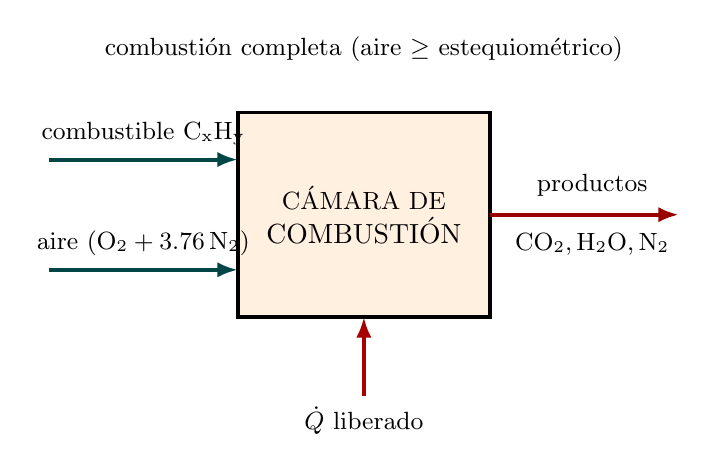
\begin{tikzpicture}[line width=1pt,>={Latex[length=2.6mm]}]
  % camara de combustion
  \fill[orange!12] (0,0) rectangle (3.2,2.6); \draw[line width=1.2pt] (0,0) rectangle (3.2,2.6);
  \node[align=center] at (1.6,1.3){\small CÁMARA DE\\COMBUSTIÓN};
  % reactivos (entran)
  \draw[->,teal!55!black,line width=1.4pt] (-2.4,2.0)--(0,2.0); \node[above] at (-1.2,2.05){\small combustible $\mathrm{C_xH_y}$};
  \draw[->,teal!55!black,line width=1.4pt] (-2.4,0.6)--(0,0.6); \node[above] at (-1.2,0.65){\small aire $(\mathrm{O_2}+3.76\,\mathrm{N_2})$};
  % productos (salen)
  \draw[->,red!60!black,line width=1.4pt] (3.2,1.3)--(5.6,1.3);
  \node[above] at (4.5,1.4){\small productos};
  \node[below] at (4.5,1.2){\small $\mathrm{CO_2},\mathrm{H_2O},\mathrm{N_2}$};
  % calor liberado
  \draw[->,red!65!black,line width=1.3pt] (1.6,-1.0)--(1.6,0); \node[below] at (1.6,-1.0){\small $\dot Q$ liberado};
  \node[align=center] at (1.6,3.4){\small combustión completa (aire $\geq$ estequiométrico)};
\end{tikzpicture}
\end{document}
